% 第六章：用户确认稿缓存，2026-10-16。章节片段，最终五页稿另行归并排版。
\section{应用场景结果展示}
为展示算法对参数退化与有限边界恢复的处理能力，本节选取球面极点、圆锥顶点及规则圆环面三角形裁剪三个案例。前两个案例取自既有固定数据，圆环面案例为本次补充的可复现正例。所有输入均先进入等参专用分支，在该分支未通过后进入一般兜底，算法不接收来源母面或预设参数图。

测试采用 Windows x64、MSVC Release 构建，每例重复三次，并对成功输出执行独立审计。整体算法耗时从统一 API 调用前计至返回后，包含识别、候选处理、边界恢复和验收，排除数据加载、来源认证、输出审计、绘图及文件写入。以三次最大耗时评价是否小于 $10\,\mathrm{ms}$，超过 $50\,\mathrm{ms}$ 的调用判为计算失败。

\begin{center}
\begin{tabular}{lccccc}
\hline
案例 & 成功且审计通过 & 连续边界上界/mm & 最大耗时/ms & $<10$ ms & $\le50$ ms\\\hline
球面 case-317 & 3/3 & $4.14\times10^{-7}$ & 6.9672 & 是 & 是\\
锥顶 case-217 & 3/3 & $5.23\times10^{-7}$ & 2.7237 & 是 & 是\\
圆环 torus-triangle & 3/3 & $2.72\times10^{-11}$ & 2.3761 & 是 & 是\\\hline
\end{tabular}
\end{center}
表中误差上界向上取整展示，均小于规定的位置容差 $10^{-5}\,\mathrm{mm}$。

\paragraph{（1）球面极点：参数退化下的边界恢复}
该案例采用双五次非有理样条表示，包含 64 个控制顶点，一条参数边在三维空间中坍缩至球面极点。球面本身在该点保持几何正则，退化发生在当前参数化中。

算法恢复球面母面及有限边界，将坍缩边显式标记为切向不适用，同时保留位置验收和其余边界的连续切向检查。三次调用均成功且通过独立审计，说明该案例中的参数退化能够在明确的验收条件下得到处理。
\begin{center}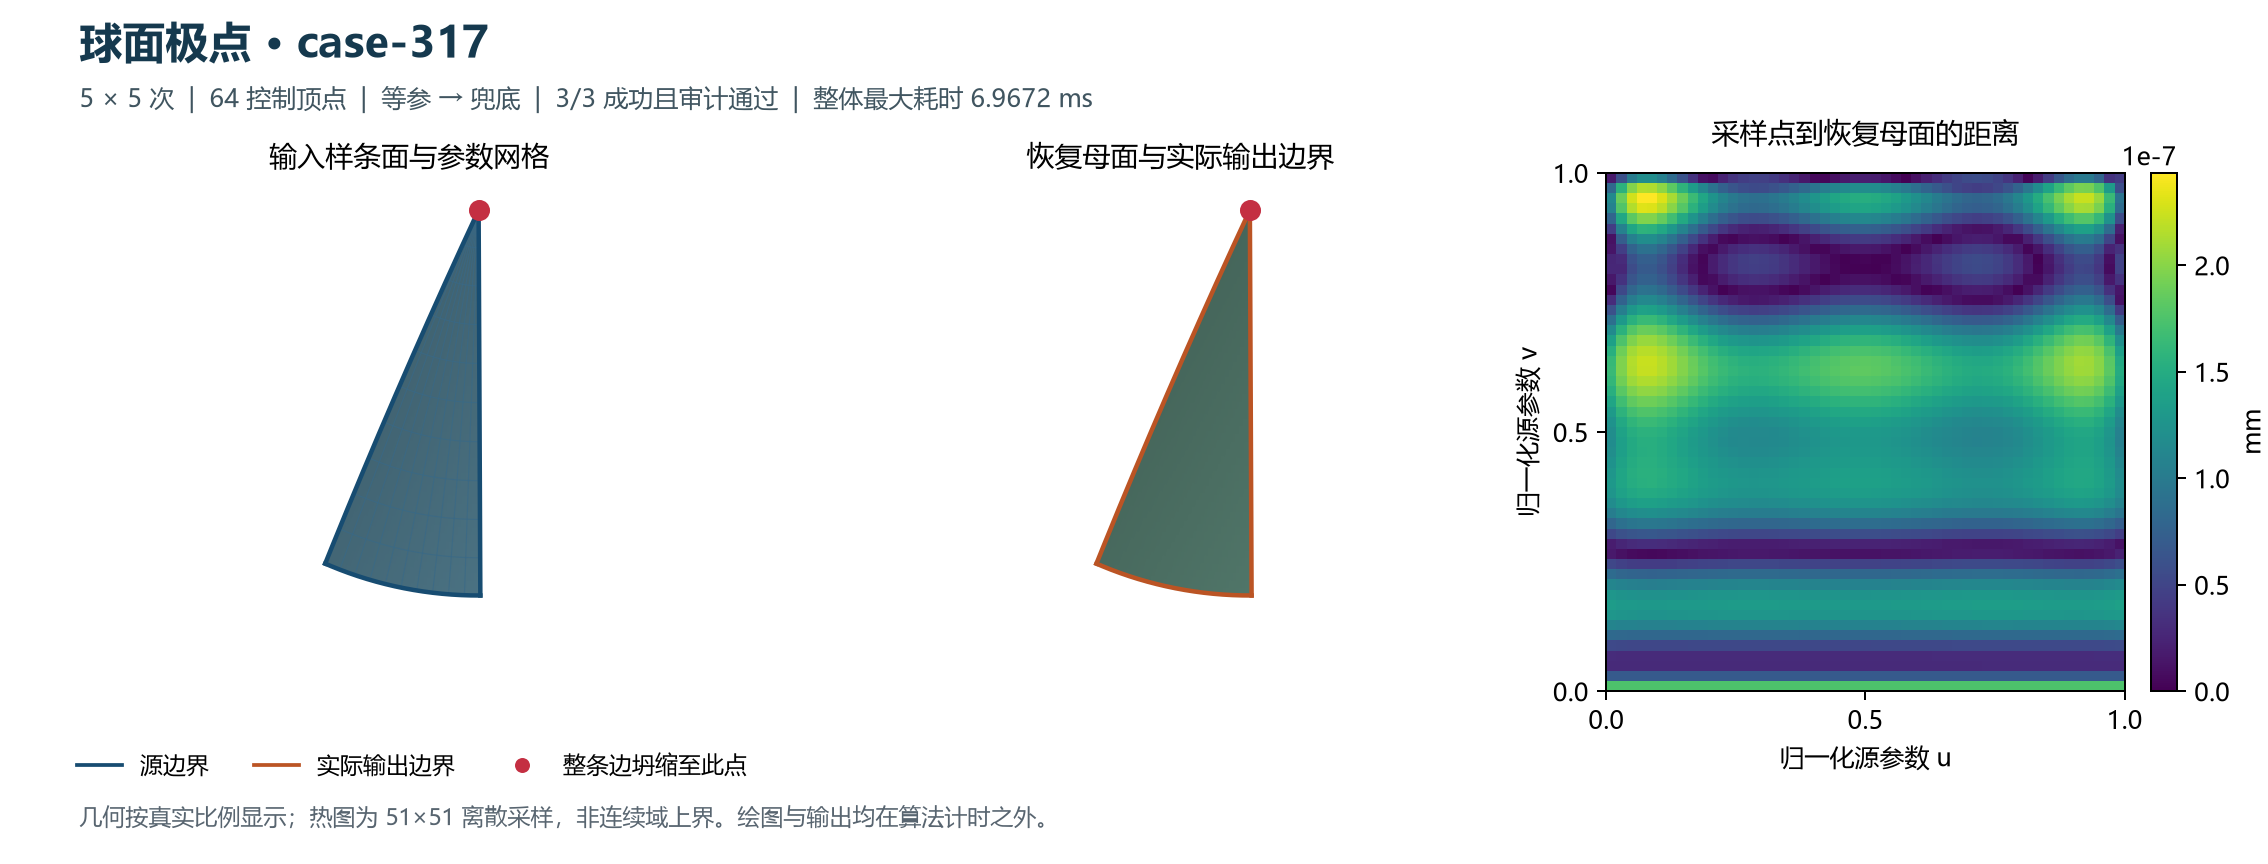
\includegraphics[width=\linewidth]{figures/sphere-317.png}\end{center}

\paragraph{（2）圆锥顶点：几何奇点处的位置保持}
该案例采用五次／三次非有理样条表示，包含 64 个控制顶点，一条参数边整体收缩至锥顶。与球面极点不同，锥顶属于母面的几何奇点，需要结合其退化结构处理边界条件。

转换结果保留了锥顶位置及其与相邻边界的连接关系，非退化边界继续接受连续位置与切向验收。独立审计同时检查实际输出曲线的共享端点和边界距离。本例整体最大耗时为 $2.7237\,\mathrm{ms}$。
\begin{center}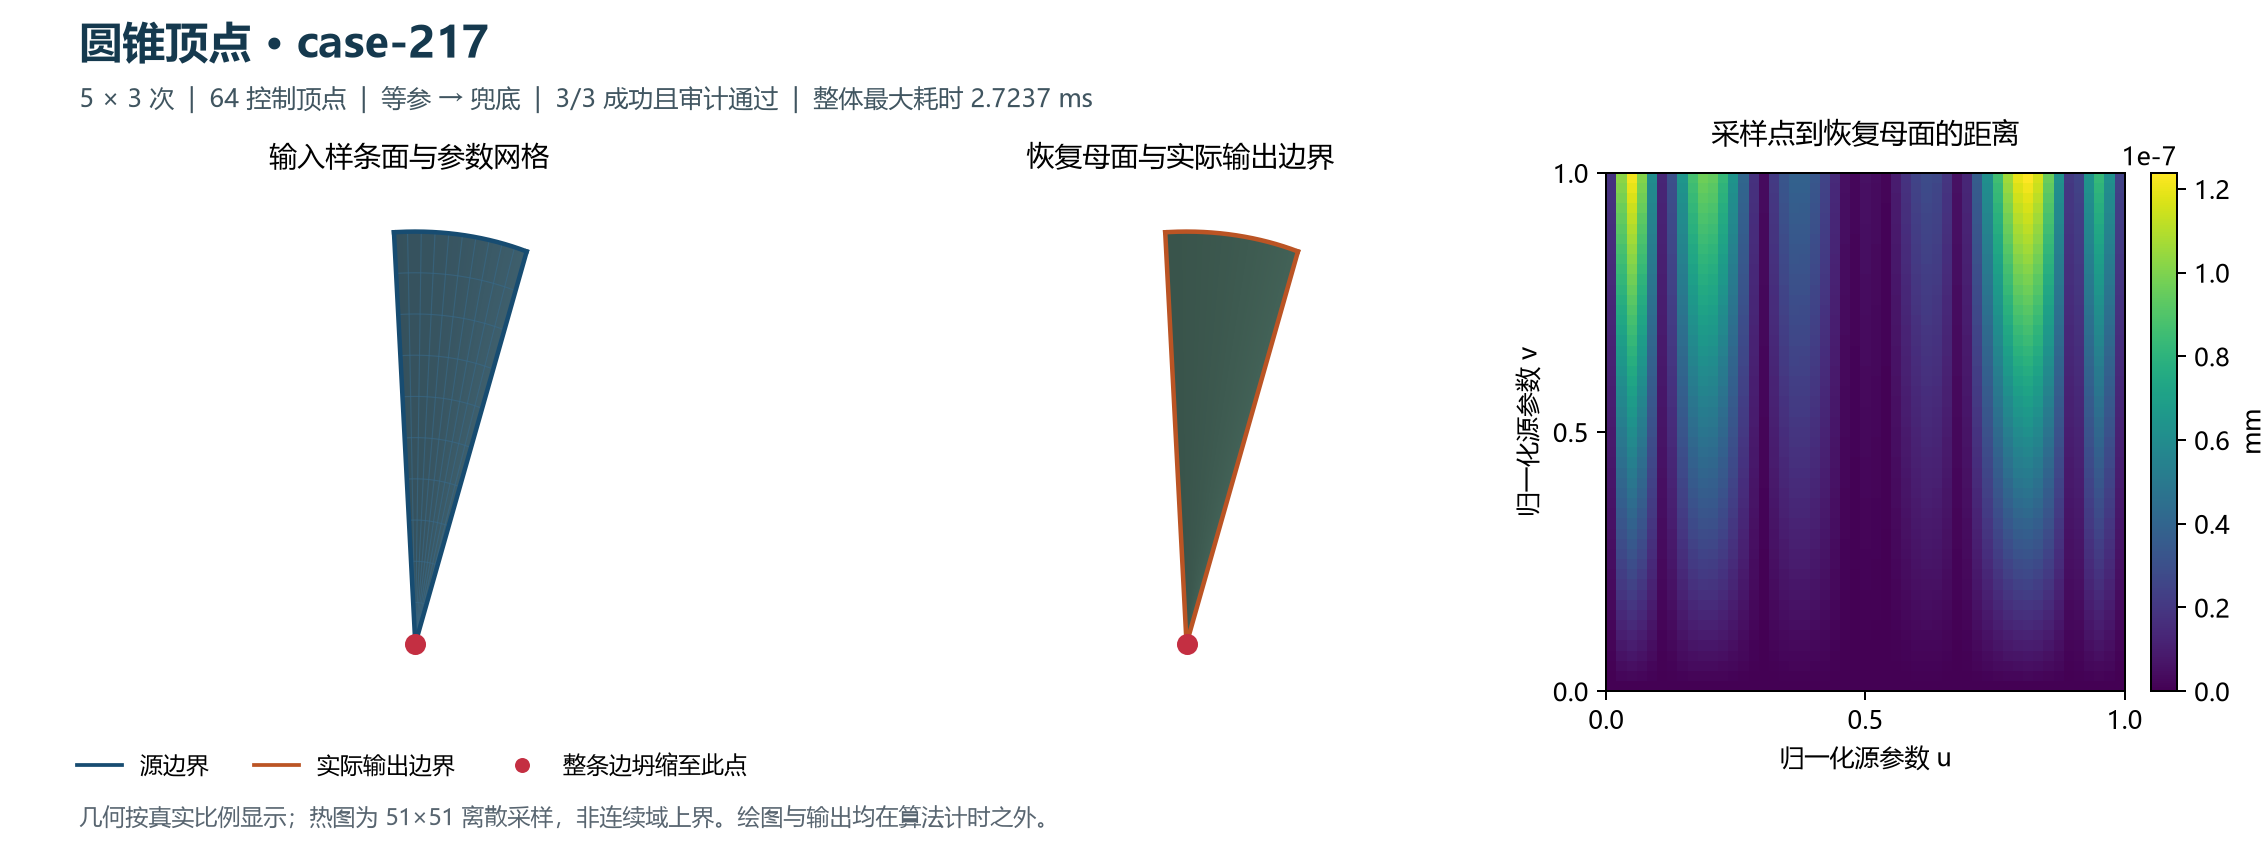
\includegraphics[width=\linewidth]{figures/cone-217.png}\end{center}

\paragraph{（3）圆环面坍缩边：正则母面上的三角形裁剪恢复}
该案例采用三次／四次有理样条表示，包含 63 个控制顶点。构造时将源参数域的一条边映射至同一空间点，使有限面片对应于目标 NURBS 参数域中的三角形区域。\textbf{这里退化的是面片参数边，规则圆环母面本身保持正则。}

算法在未获得预设母面和参数图的条件下，恢复圆环面参数、三角形裁剪区域及三维边界曲线。该结果展示了处理范围从常规四边形面片延伸至满足退化判据的三角形面片的能力，而不必为维持四边结构人为保留一条短边。
\begin{center}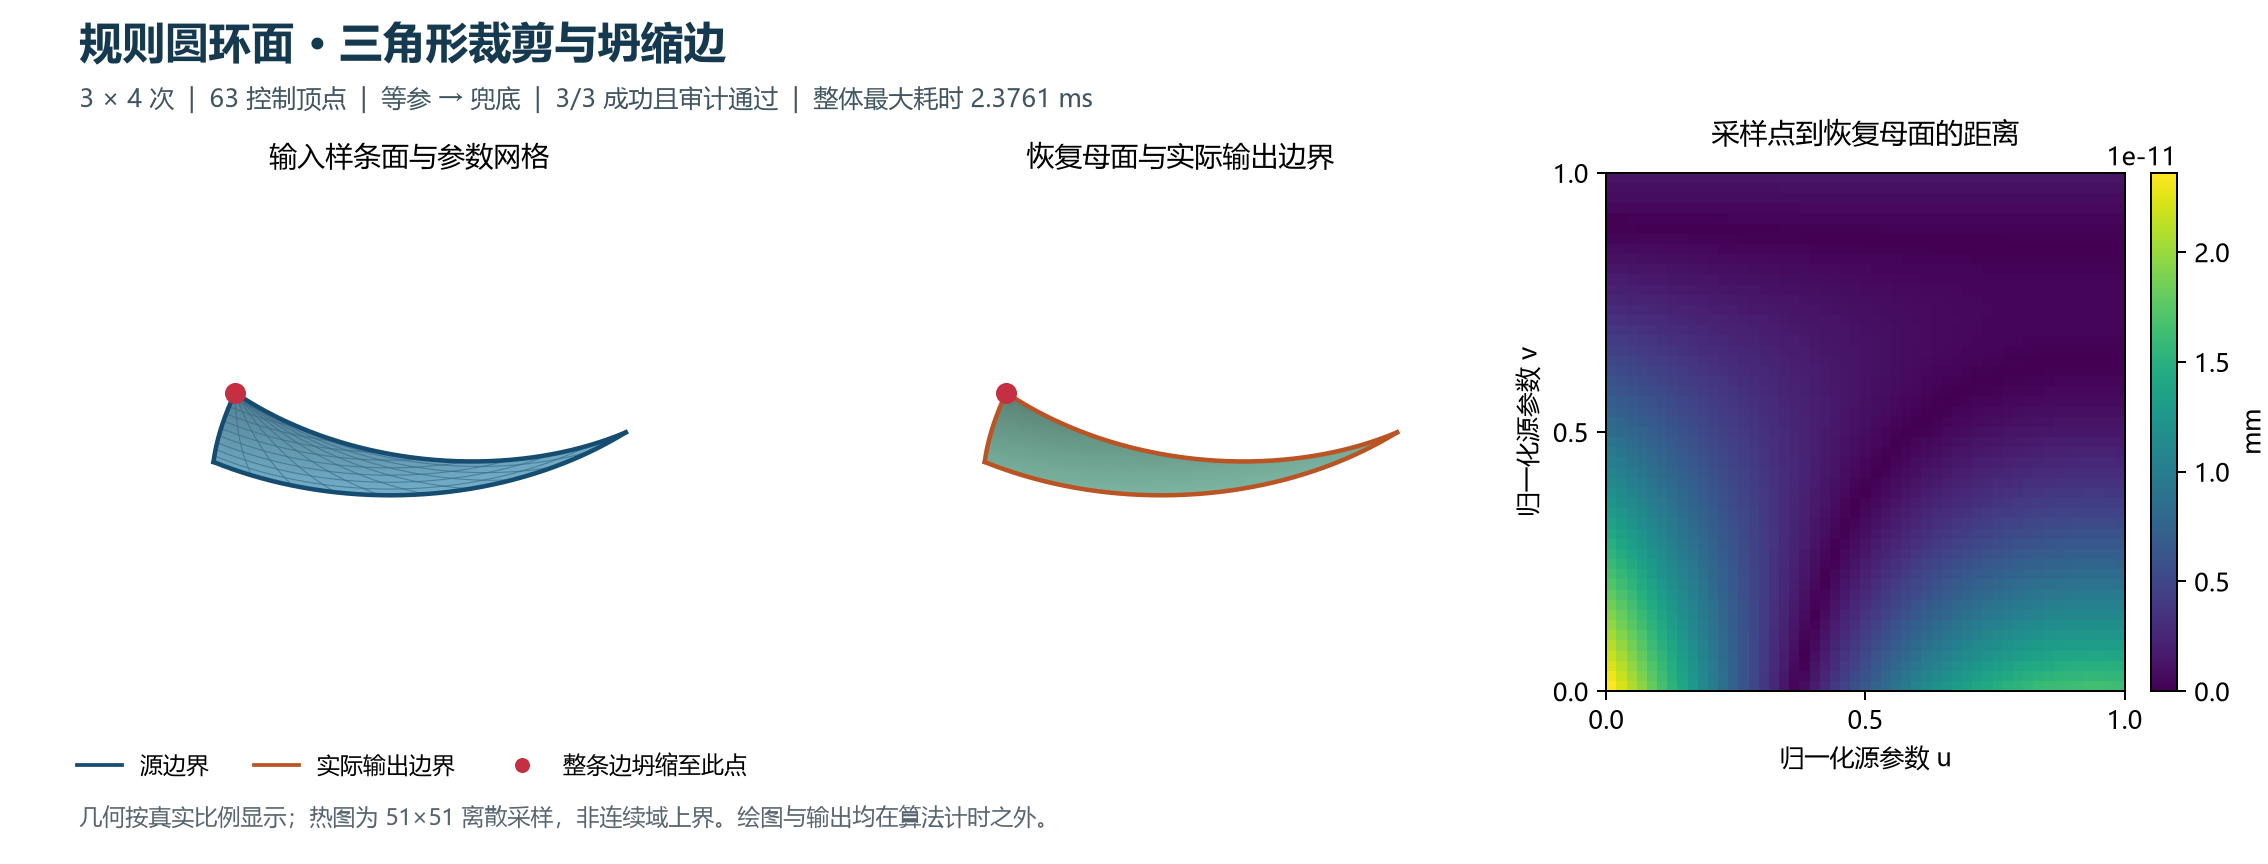
\includegraphics[width=\linewidth]{figures/torus-triangle.png}\end{center}

图中左侧为实际输入曲面及参数网格，中间为恢复母面的有限区域和实际输出边界，红点标记整条边的坍缩位置。右侧热图展示 $51\times51$ 源参数采样点到恢复母面的距离，各图采用独立色标；热图用于观察误差分布，连续边界误差以上表的认证上界为准。

三个案例均未使用微小分段切向豁免，且母面优化迭代数均为零，因此主要验证分支衔接、边界恢复及整边退化处理能力。上述定向结果不替代全量回归，既有全量批次仍存在预算失败案例。
% 证据：docs/testing/introduction-cases-2026-10-16/README.md
